% ------------------------------------------------------------- 
% Arquivo :  relatório modelo                                        
% ------------------------------------------------------------- 
% O percentual(%) serve para incluir comentários: 
% tudo o que fica à direita dele não é interpretado pelo LaTex
% Linhas e espaços em branco também **NÃO** são
% interpretadas pelo LaTex

%% As intruções seguintes são o cabeçalho e devem estar antes do
%% \begin{document}

%\documenclass: mandatorio, indica o tipo/formato de documento
\documentclass[brazilian,12pt,a4paper,final]{article}
%\documentclass[brazilian,a4paper,final]{article}
% tamanhos de fontes: 10pt, 11pt ou 12pt
% opções de estilo (padrões): article, report, book, slide, letter (artigo, relatorio, livro, apresentação de slides, carta)

%% Pacotes extras (opcionais):
% *geometry* determina a geometria da página:
%	a4paper: tamanho físico do papel: A4
%	tmargin=1in: margem no topo = 1 polegada
%	bmargbin=0.8in: margem no fundo = 0.8 polegadas...
\usepackage[a4paper]{geometry}
\geometry{verbose,tmargin=1in,bmargin=0.8in,lmargin=1in,rmargin=0.8in}

% *babel* contem as regras de ifenização
\usepackage[brazil]{babel}

% *t1enc* permite o reconhecimento dos acentos inseridos com o teclado
%\usepackage{t1enc}

% *inputenc* com opção *utf8* permite reconhecimento dos caracteres com codificação UTF8, que é padrão dos editores de texto no Linux. Isso permite reconhecimento automático de acentuação.
\usepackage[utf8]{inputenc}

% *graphicx* é para incluir figuras em formato eps 
\usepackage{graphicx} % para produzir PDF diretamente reescrever esta linha assim: \usepackage[pdftex]{graphicx}

% Os pacotes da AMS (American Mathematical Society) abaixo permitem usar
%	recursos mais avançados de formatação de equações.
% Ver ambientes \begin{align*} \end{align*}
%	e \begin{align} \end{align} nos exemplos abaixo.
\usepackage{amsmath}
\usepackage{amsfonts}
\usepackage{amssymb}

% *color* fontes soloridas
\usepackage{color}
%%% fim do cabecalho %%%

\pagestyle{empty}
% Veja a nota de rodapé no título.
\title{Métodos Computacionais da Física A\footnote{Nota de rodapé no título: este trabalho reproduz...}}
\author{Aluno: nome - Matrícula: número \\ IF-UFRGS}

\begin{document}
\maketitle % Este comando gera o cabeçalho do artigo/relatório.
\begin{abstract}
Descrever de forma sintética o problema 
e os resultados.
% as quebras de linha coma a de cima não são interpretadas
% para forçar quebra de linha deve ser deixada uma linha em branco
\end{abstract}

%Abaixo podem ver como se deve colocar letras acentuadas ou latinas se
%o pacote *t1enc* não dfosse usado 
\section{Introdu\c{c}\~ao} % Ou Introdução
% Aqui a Introdução \c{c} e \~a  é a forma standard  de escrever
% carateres ASCII extendidos (acentos, etc), porem com o pacote t1enc
% declarado acima podemos escrever diretamente ç em lugar d \c{c}, etc
Pequeno histórico do problema. 
Explicar porque o trabalho é relevante.

\section{Método}
% Aqui o Método 
Detalhes sobre o método utilizado \cite{Kauffman_book},
%procure ao final do texto a referencia a esta bibliografia.
demonstrações de porque ele funciona.  Limites analíticos, etc.


Exemplo de fórmula matemática sem numeração:
\[
\int_{0}^{\infty} f(x) dx
\]

% Exemplo de fórmula numerada.  O número é gerado automaticamente.
% A fórmula tem um rótulo (label) chamado "gauss", que permite a
%	realização de referências cruzadas ao longo do texto.
Exemplo de fórmula matemática (1 linha) com numeração:
\begin{equation}\label{gauss}
	\int_0^\infty e^{-x^2} = \frac{\sqrt{\pi}}{2}
\end{equation}

Referência cruzada à fórmula acima: ... de acordo com (\ref{gauss}), a integral imprópria da função gaussiana é conhecida.

% Exemplo de mais de uma linha de equações com o ambiente align* da AMS.
% Note o alinhamento com o símbolo "=", obtido com &
% Cada linha da equação é finalizada com o comando "\\"
Exemplo de diversas linhas de fórmulas, sem numeração:
\begin{align*}
	\int_0^1 \left(1-\sqrt{x}\right)^{p-1} dx &= \frac{2}{p(p+1)} \\
	\int_0^\infty \frac{e^x - e^{-x} + 2}{\left(e^x - 1\right)^2} x^2 dx &= \frac{2}{3} \pi^2 - 2
\end{align*}

% Exemplo de mais de uma linha de equações com o ambiente align da AMS.
% Note o alinhamento com o símbolo "=", obtido com &
% Cada linha da equação é finalizada com o comando "\\"
% Todas as linhas são numeradas, exceto se o último comando for 
%	"\nonumber".
% Rótulos 
Exemplo de diversas linhas de fórmulas, alternando numeração:
\begin{align}
\int_0^\infty e^{-\beta x} \left(1 - \cos ax\right) \frac{dx}{x} &= \frac{1}{2} \ln 
	\frac{a^2 + \beta^2}{\beta^2} \label{for2_1} \\
\int_0^\infty J_\nu \left(bx\right) dx &= \frac{1}{b} \nonumber \\
\int_0^\infty x K_\mu \left(ax\right) J_\mu \left(bx\right) dx &=
   \frac{b^\mu}{a^\mu \left(b^2 + a^2\right)} \label{for2_2}
\end{align}

Referências às fórmulas acima no texto: ... a fórmula (\ref{for2_1}) envolve somente exponenciais, enquanto que a fórmula (\ref{for2_2}) envolve funções de Bessel.

Exemplo de lista numerada:
\begin{enumerate}
  \item{ primeiro }
  \item{ etc }
  \item{ etc }
\end{enumerate}

% O verbatim faz o latex ignorar a formatação: ai SIM os espaços e
% linhas em branco contam
% É util para trechos de código Fortran por exemplo
\vspace{0.3cm}
Exemplo de texto sem formatação para código {\bf FORTRAN} por exemplo
Veja o %\bf acima

\begin{verbatim}
...
Read (*,*) a, b, t

 Do i=0,t
    b(i) = a*c(i)
 End do
...

\end{verbatim}

\section{Resultados}
\vspace{2cm}
 Aqui os resultados, sua interpretação.

% Aqui incluimos uma figura
% Para testar este comando devem criar uma figura em formato
% postscript encapsulado (eps) e deve ter o mesmo nome que aparece entre chaves
% no caso ``fig.eps'' 
Incluindo uma figura em formato PDF

\begin{figure}[hbtp]
\begin{center}
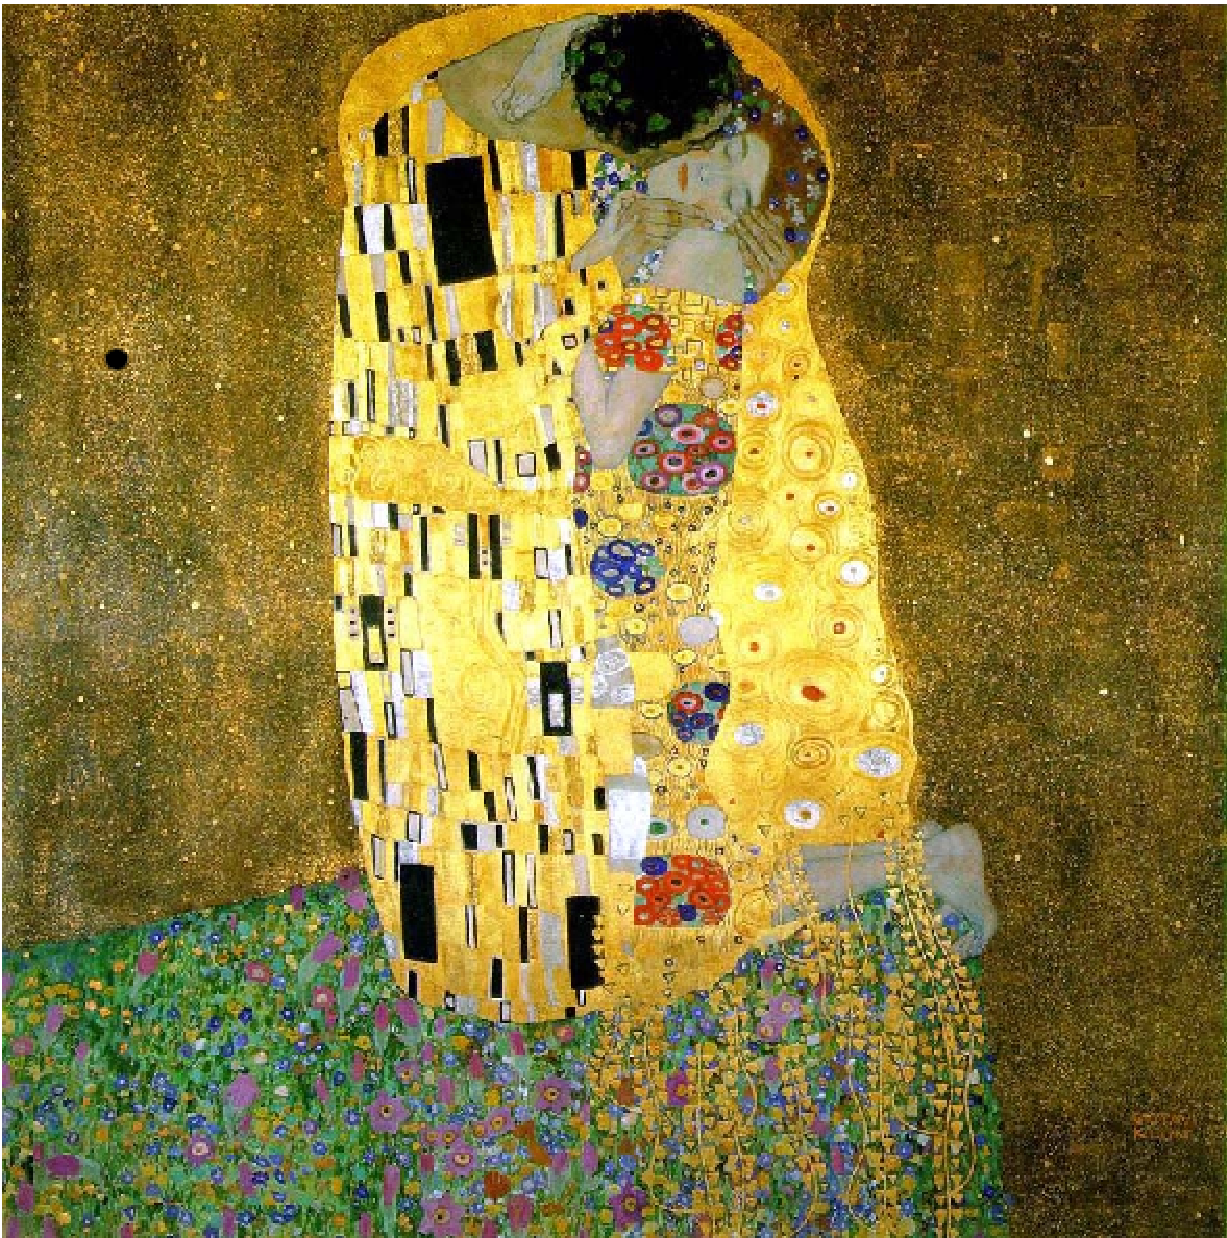
\includegraphics[width=8cm]{klint.pdf}
\caption{Coloque aqui as legendas}
\label{fig}
\end{center}
\end{figure}
\vspace{0.5cm}

\begin{figure}[htbp]
\begin{center}
\rotatebox{-90}{\resizebox{8.0cm}{!}{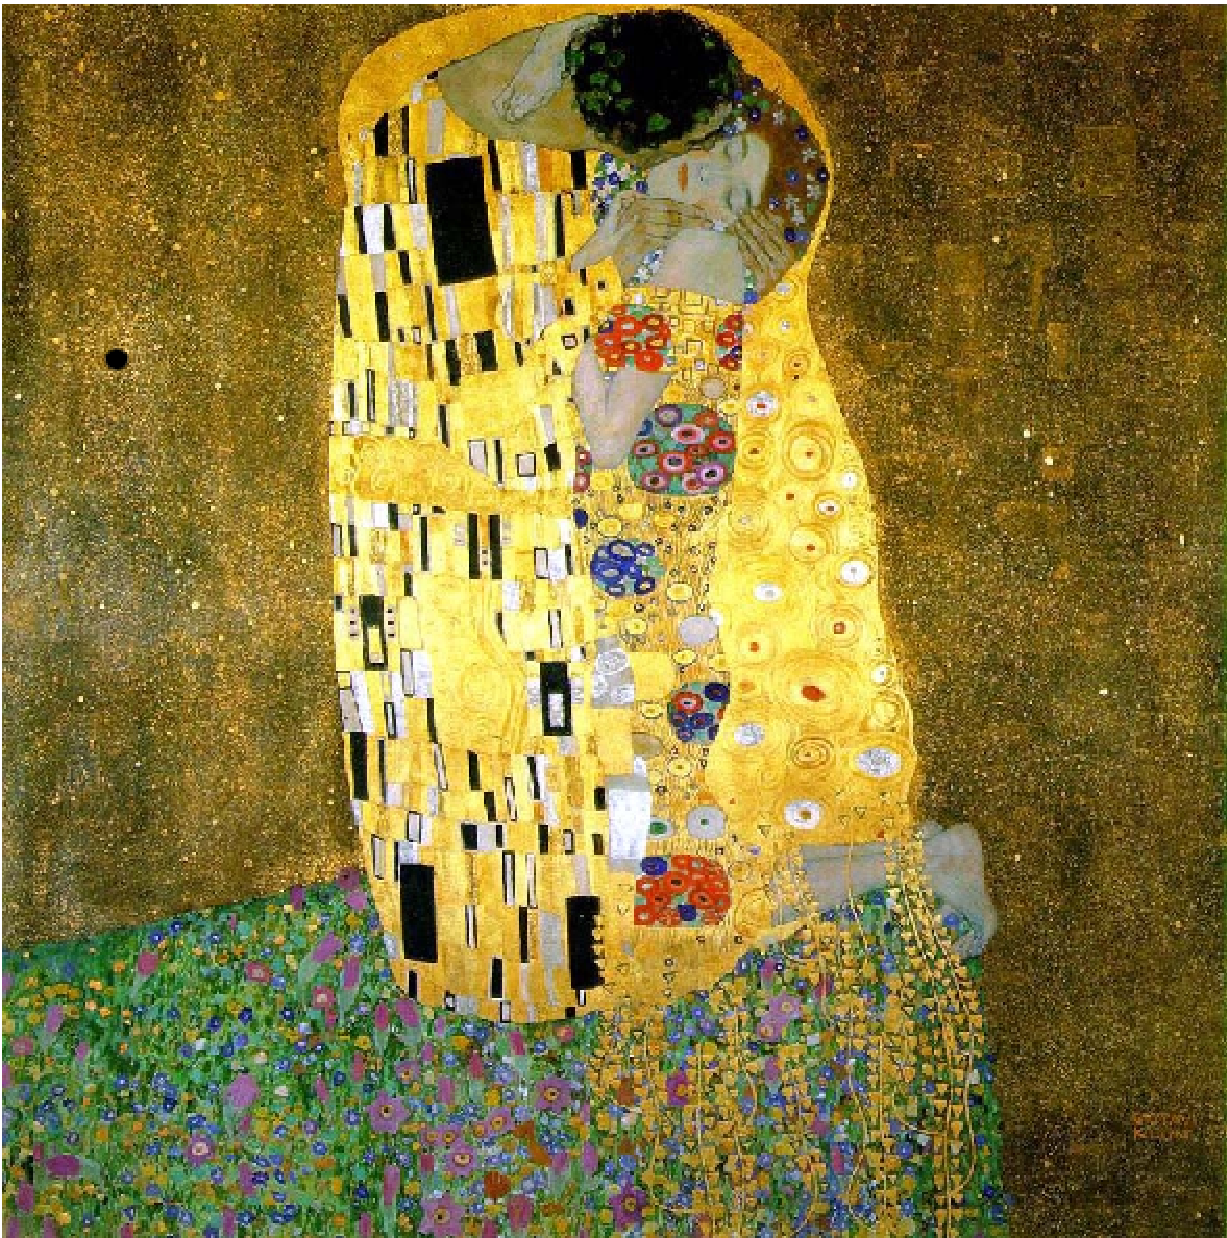
\includegraphics{klint.pdf}}}
\caption{Legendas}
\label{fig_rotacao}
\end{center}
\end{figure}



Incluindo uma tabela:
\begin{table}[h]
\begin{tabular}{||l|c|r||} \hline
tempo& posição & velocidade\\
\hline
0 & 1 & 3\\
 1 & 2 & 4\\
 2 & 3 & 5\\
 \hline
 \end{tabular}
 \caption{A tabela mostra os valores de tempo, posiçao e velocidade do
{\ldots} }
\end{table}

\section{Conclusões}
Recolocar resumidamente o problema, os resultados, as comparações \cite{Wolfram_book} com outros
trabalhos e as perspectivas futuras que o trabalho abre.

A referência \cite{Ramos+18} consiste em um trabalho publicado na Revista Brasileira de Ensino de Física.

{\color{red} Este é um modelo geral, quando for utilizá-lo para um trabalho
específico leve em consideração as necesidades desse trabalho,
cuidando de omitir ou comentar com \% \% as seções que não
se apliquem.}

\begin{thebibliography}{99}

\bibitem{Kauffman_book}
S.~Kauffman, {\em The Origins of Order: Self-Organisation and
Selection in Evolution}, (Oxford University Press, 1993).

\bibitem{Wolfram_book}
S.~Wolfram, {\em Theory and Application of Cellular Automata},
(World Scientific, Singapore, 1986).

\bibitem{Ramos+18}
I. R. ~O. Ramos, J. P. ~M. Braga, J. V. ~A. Ataíde, A. ~P. Lima, L. Holanda,
Revista Brasileira de Ensino de Física \textbf{40}, e5408 (2018).

\end{thebibliography}

\end{document}

